\section{Device Driver}
\subsection{Device Driver Model}
\subsubsection{Introduction} 
Nowadays most of operating systems support various of devices, and these device drivers run in kernel space which can response to the applications immediately. But there is a big problem in this model, device drivers and kernel run in the same address space will make the kernel unstable. So in some real-time embedded operating system, device drivers run as threads which are activated by interrupts. L4 and QNX is using this device driver model. In this kind of device driver model, appications must send request through the IPCs to the device driver sevice routine if they want to use the device. So it is thought less efficiency than the first model, but it is proved that this viewpoint is incorrect. 
\\
This model is mainly used in micro-kernel systems, but XtratuM is a nano-kernel system. Instead of the threads, domains are running above the core. Domains have their separated kernel space and user space. So the device drive is running as a domain in the system, and other domains use IDC (Inter-Domain Communication) tools to communicate with the device driver domain. There is the architecture of XtratuM device driver model. 
\begin{center}
	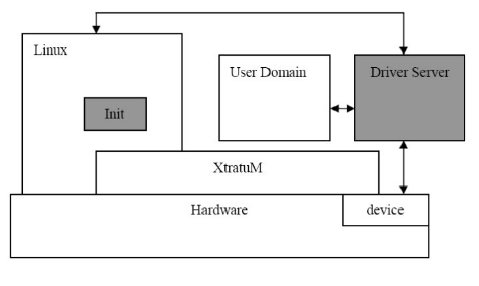
\includegraphics[width=0.8\linewidth]{graph/dev01.jpg}
\\
	Fig1 : XtratuM Device Driver Model Arcihtecture
\end{center}
As we see in the graph, there are two parts of a XtratuM device driver. One is the initialization component in Linux and another is the real-time device driver run as a domain in the system. The initialization component in Linux continue to use the code provided by Linux which increase the reuse of the code. In the real-time device driver component, there are two functions: interrupt handle and the real-time device driver. The domain of device driver will be idle in the system until it is triggered by the interrupt. 
\subsubsection{Development}
When we start to development a device driver in the system, there are two things to consider: resource management in Operating system and hardware. The first part of the device driver communicates with the operating system, it prepares the resources for the hardware management part. This part includes the resource requirement and management from the operating system, such as memory, interrupt handle and I/O ports etc. As we known, XtratuM only take care of the critical resource from Linux, such as memory, timer and interrupt. So this part uses the functions provided both by Linux and XtratuM. It will run as a module in Linux at the Linux kernel space. The second part communicates with a particular hardware, it takes care of device access and provides interface to the user in the system. This part runs as a domain in XtratuM and communicates with other domains by inter-domain communication tools, such as fifo and shared memory.
\\
Before we start to explain how to add a device driver in the system, we should know the structure of XtratuM source tree, it is shown in the figure as following:
\\
\begin{center}
	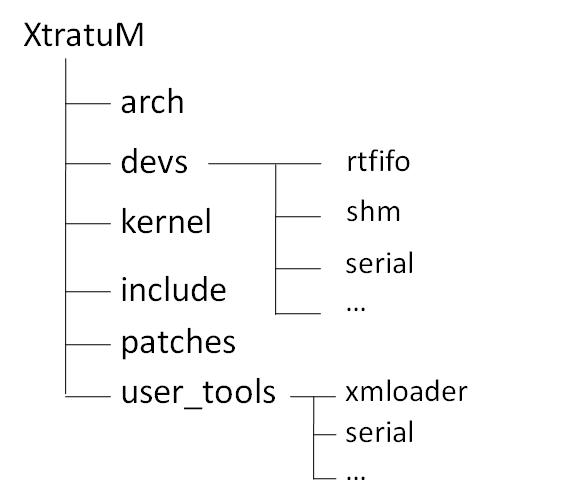
\includegraphics[width=0.8\linewidth]{graph/dev02.jpg}
\\
	Fig2 : XtratuM source code structure
\end{center}
There are two import directories when you add a device driver in XtratuM: devs and user\_tools. We put the first part of device driver under the directory devs and called it initialization component, and the second part under the directory user\_tools called device driver server.
\\

\begin{itemize}
\item{Initialization component}
\\
We put different device drivers in different directories as shown in the above figure. The access interface from Linux side is also implemented under the directory following the device class given by Linux kernel, such as character devices and block devices. The access interface make it is possible to access the device from Linux user space. So in the example of serial port device driver, there are two parts in this directory: initialization component and Linux interface.
\\
As we mentioned above, the initialization component should request three kinds of resources from the system: I\/O port allocate, smemory management, irq handler and device register. And we also need to register the device to XtratuM in this componenet.

\begin{itemize}
\item{I\/O port allocate}
\\
I\/O port is used by device driver to communicate with the hardware. It is managed by Linux kernel. Here is the functions provided by Linux kernel.
\begin{verbatim}
#include <linux/ioport.h>
struct resource *request_region(unsigned long first, unsigned long n,
const char *name);
\end{verbatim}

The parameters of this function tell the kernel that the device driver wants to use n ports from the first, and the name is the symbol of your device driver. It will return a address of resource structure in the normal condition. If it returns a NULL, the device driver will not use the ports it is expected. So check the return value of request\_region() in your device driver.
\\
There is also a function to check the use status of a set of ports.
\begin{verbatim}
int check_region(unsigned long first, unsigned long n);
\end{verbatim}
It will check the use status of n ports from first. But there is a possibility that the ports is allocated before the device driver request the ports after checking it. This function is not commended to use.\\
And when everything is done, you should release the resource to system by using the function release\_region(). The parameter start is corresponding with first.
\begin{verbatim}
void release_region(unsigned long start, unsigned long n);
\end{verbatim}

\item{irq handler allocate}\\
The irq handler can be allocated by the functions in Linux kernel. 

\begin{verbatim}
#include <linux/interrupt.h>
int request_irq(unsigned int irq,
        irqreturn_t (*handler)(int, void *, struct pt_regs *),
        unsigned long irqflags,
        const char *devname,
        void *dev_id);
\end{verbatim}
This function is used to fill the irq\_action structure in irq description array. The structure is as following. The parameters are corresponded with the items in the structure.
\begin{verbatim}
 struct irqaction {
    irq_handler_t handler;   /* point to the irq server routine */
    unsigned long flags;     /* interrupt flags */
    unsigned long mask;      /* interrupt mask*/
    const char *name;        /* name of the I/O device*/
    void *dev_id;            /* device identification mark */
    struct irqaction *next;  /* point to the next structure */
    int irq;                 /* the irq number required */
    struct proc_dir_entry *dir; /* point to the directory of /proc/irq/n */
};
\end{verbatim}
This is a reuse of Linux functions, but there is a different from the Linux in our device driver model. We use irq number to identify the device driver instead the dev\_id in Linux. So in your device driver you can fill the last parameter with NULL. And the flag has these values:
\begin{itemize}
\item{SA\_INTERRUPT}\\
This kind of interrupt server routine will be executed with interrupts disabled .\\

\item{SA\_SHIRQ}\\
This interrupt can be shared between devices. \\

\item{SA\_SAMPLE\_RANDOM}\\
This means the devices must can return random numbers which can be use in the entropy pool used by /dev/random and other device like it.This bit indicates that the generated interrupts can contribute to the entropy pool.\\
\end{itemize}
As the I\/O ports, after you use the irq\_handler you should release the resource by free\_irq(). Here use the irq number to identify which irq\_handler should be released.
\begin{verbatim}
void free_irq(unsigned int irq, void *dev_id);
\end{verbatim}

\item{Memory allocate}\\
The memory allocate is using the functions provided by Linux to get a block of physical memory and using the function provided by XtratuM to implement the memory map from the separate domain space. It can map the domain space to the IDC, such as fifo and shared memory, which will provide the communication mechanism between device driver and domains using the device. \\
\begin{verbatim}
#include <linux/mm.h>
unsigned long  __get_free_page(unsigned int flags);
void free_page(unsigned long addr);
\end{verbatim}
\_\_get\_free\_page() can allocate a whole page of physical memory for device driver, and the flags in \_\_get\_free\_page are as following:\\
\begin{itemize}
\item{GFP\_KERNEL}\\
This means the memory allocated is a normal for kernel which can sleep.\\

\item{GFP\_ATOMIC}\\
This kind of memory is allocated for something outside of the process context just like interrupt handlers, it can not sleep.\\

\item{\_\_GFP\_DMA}\\
Choice this one if your device can access memory through ISA directly.\\

\item{\_\_GFP\_HIGHMEM}\\
This flag means the page is allocated for high memory.\\
\end{itemize}
After get the physical memory, you still need to build the memory map from the hardware to the device driver server domain. 
\begin{verbatim}
// Virtual address to page directory entry
#define va2pd(vaddress) (vaddress >> PGDIR_SHIFT)

// Virtual address to page table entry
#define va2pt(vaddress) ((vaddress & 0x3FF000) >> PAGE_SHIFT)

// Page directory and page table to virtual address
#define pdpt2va(pd, pt) ((pd << PGDIR_SHIFT) | (pt << PAGE_SHIFT))
\end{verbatim}

\item{Device register}\\
The device driver register function in XtratuM is implemented in xmdev.c under directory XtratuM\_PATH\/kernel. 
\begin{verbatim}
#include <xmdev.h>
int xm_dev_register(int devid, xm_dev_t *dev);
int xm_dev_unregister(int devid);
\end{verbatim}
The devid here is the device driver number defined in the xmdev.h, you should add it when you implement your own device driver. dev is a structure of your device driver it defined the operations and parameters of your device drive. You should initialize it before you use it.
\begin{verbatim}
#include <xmdev.h>
typedef struct
xm_dev_struct
{
	int devid;
	int (*dev_map_handler)(unsigned long, unsigned long, 
			unsigned long, void *);
	int (*dev_unmap_handler)(unsigned long, unsigned long, 
			unsigned long);
	int (*dev_ioctl_handler)(unsigned long minor, 
			unsigned long cmd, void *);
	int client;
} xm_dev_t;
\end{verbatim}
This part only requires the resources from the system, and the handler routine will implement in device driver server domain.\\
So the pseudocode is like this:
\begin{verbatim}
xm_dev_t  xm_dev = {};
struct resource *dev_res;
int xm_devl_xm_init(void)
{
	 ();
	init_xm_dev_parameter();
	xm_mem_map();
	xm_dev_register();
	xm_request_irq();
}
void xm_serial_xm_exit(void)
{
	xm_free_irq();
	if(xm _dev.client > 0) {
		XMBUG();
		return;
	}
xm_dev_unregister();
	xm _mem_free();
	release_region();
}
\end{verbatim}
\end{itemize}

\item{Device driver server}
\\
Device driver server is run as a domain in XtratuM, we put this under the XtratuM\_PATH\/user\_tools. In this component we will implement the access functions, such as read\/write functions through the IDC, irq handler routines and the scheduler functions. You can set up your own scheduler queues with your scheduler method in this component.
\\
\begin{itemize}
\item{I\/O ports}
\\
The access functions is as following:
\begin{verbatim}
#include <xmdev.h>
#include <asm/io.h>
unsigned inb(unsigned port);
void outb(unsigned char byte, unsigned port);
\end{verbatim}

The parameter port is the port which is required in the initialization component, and the byte means the size you want to write to the port.\\
\item{irq handler}

Based on the different parameter passed by the function, you should implement different access method for your device.\\
\item{Memory access}\\

You should choose an inter-domain communication tool to support your server domain to communicate with the user domains. Now there are two IDCs in the system: fifo and shared memory. The first one is suitable for the short messages and the second one is suitable for big block of data which will be modified partly.\\
\end{itemize}
\item{Add the event handler}
\\
Add the event handler in the structure of event\_handling\_struct in include\/events.h.
\end{itemize}
\subsection{XM/Serial Driver}
\subsubsection{About XM/Serial Driver }
1)  WHAT IS XM/SERIAL DRIVER
\\
Xm/serial means that do communication through serial ports based on XtratuM and the xm/serial driver is the thing that can support user to communicate by serial port. It meets the real-time requirement. In XtratuM, one part of XM/SERIAL DRIVER runs as a XtratuM domain. so the developer can use the XM/SERIAL DRIVER to do communication through serial ports to meet their own needs by modify the driver domain.
\\
2)  XM/SERIAL DRIVER CHARACTERISTICS
\\
UART is used to connect a number of standards to support the Universal Serial communications equipment ,so the driver developer only needs to write driver for UART .
\\
	In Xtratum, the uart device is divided into two parts, one is loaded into kernel as module which is used to request resources for serial device, such as locating memory for FIFO, the UART's address space and so on, the other is loaded as a domain which initialize the device driver. There is only one device domain, reads from serial fifo or write data to serial fifo, so there is no concurrent problem.
\\
	There are 16 pairs of Lock-Free FIFO for IDC(inter-domain-communication), There are two fifos for each pair and the fifo is un-direction, one fifo send data from guest domain to server domain and the other fifo is opposite. Each pair of fifo can not be shared by multiple guest domains.
\\
	An scheduler based priority is provided in the uart device driver server. There will be an interrupt when Transmitter Holding Register is empty and this interrupt will trigger uart device driver domain which will choose the nonempty fifo which has highest priority an dada source by scheduler. If there is no data in all FIFOs, the Transmitter Holding Register's null value interrupt will be shielded and the null value interrupt can start when guest domain write data to fifo.
\\
	The serial driver domain was defined in serial.c in which the serial port address and baudrate defined, such as 
"static uart\_dev\_t uart=\{4,0x3f8,0,115200\}" ,the meaning of the four parameter is irq, port address, the parity and baudrate. Another important function is vuart\_device\_init(void). In this function, the address for 16 fifos which used to make communication are located.
\\
3)  THE USE OF XM/SERIAL DRIVER 
\\
The UART driver domain can initialize the hardware when device running and support the implementation of the special operation for the device. One of its importandt use is to serve the guest domains to meet their communication needs and developers can use it easily to communicate with other domain by serial ports.
\\
	One of its benefits for the driver domain is that it can decrease the threat to the kernel, it runs as domain just like a thread and
 the developer can modify the driver domain by modifying the serial.c, such as modifying baudrate in 
"static uart\_dev\_t uart=\{4,0x3f8,0,115200\}" and another parameters.

\subsubsection{Using XM/Serial Driver}
1) About XM\/Serial Driver
\\
Here will introduce how to build guest domains and use them to do communication by serial ports. The maximal device number and minimal device number is fixed in the guest domains. The maximal port device number is 2,the minimal number is to represent different fifos,
\\
When the guest domain is loaded, it will call suspend\_domain() to initialize device, then the guest domain will set the attribute for serial port, such as priority and speed and so on.
\\
There are functions dom\_serial\_fifo\_write() and dom\_serial\_fifo\_read() in uart domain and they realize how to write and read dada detailed. so you have to add these two function in your guest domain. The function rt\_serial\_write(const char *src, int size) which calls dom\_serial\_fifo\_write() is used to write data whose address is src to the serial port and its length equals to size. Function rt\_serial\_read(char *dst, int size) which calls dom\_serial\_fifo\_read() is used to receive data from the serial port , the data¡¯s length equals to size. So the developer only have to know how to use rt\_serial\_write(const char *src, int size) and rt\_serial\_read(char *dst, int size) and that is enough. 
\\
	As gived example on this version XM/eRTL, there are two fundamental examples, developer can change the baudrate by the parameter
 for function serial\_device\_init(unsigned init ttys, long  baud), the ttys represents fifo which 0<=ttys<16. In the kmain(), developers 
can do what they want to do, such as sending "Hello, XM/eRTL" to another computer by serial ports, but XM/eRTL has to be installed on the 
other computer and the uart driver domain has been loaded.
\\
	Generally speaking, what developers have to do is to give parameters to serial\_device\_init(unsigned init ttys, long  baud) , rt\_serial\_read(char *dst, int size) and rt\_serial\_write(const char *src, int size).
\\
	So if you want to use the UART driver to do serial port communication, firstly, the UART Driver domain should be loaded,
\\
2)  XM/SERIAL DRIVER DOMAIN EXAMPLE
\\
To do communication through serial ports, you should first make sure you have installed XM/eRTL and have loaded the uart driver domain 
"serial.xmd". Next, you can build your own guest domain.,
\\
Here is an simple example will be introduced. The server will send the message " UART TEST SCCUCESSFULLY " to the client and the client will display what it has received(Both server.c ,client.c and some comments you can see them at Appendix III).
\\
	In the server domain, the function kmain() which is in server.c is as following:
\lstset{language=C}`
\begin{lstlisting}
static char string[40] = {"UART TEST SCCUCESSFULLY\n"};
							  .
int kmain (void) 
{
   struct xmitimerval req = {{0, 200000}, {0, 0}};
   long baud =115200;
   int ret;
   ret = serial_device_init(my_Console_ttyS, baud);  
		//initialize device with 
		// your fifo number and baudrate
   set_timer(&req, 0);
   install_event_handler(0, timer_handler);
   unmask_event(0);
   enable_events_flag();
   suspend_domain (0, 0);
   rt_serial_write(string,40);
   return 0;
}			
\end{lstlisting}
	In the client domain, the function kmain() which is in client.c is as following:
\lstset{language=C}
\begin{lstlisting}

static char string[100];
				    		  .
int kmain (void) 
{
   struct xmitimerval req = {{0, 200000}, {0, 0}};
   long baud =115200;
   int ret;
   ret = serial_device_init(my_Console_ttyS, baud);
   set_timer(&req, 0);
   install_event_handler(0, timer_handler);
   unmask_event(0);
   enable_events_flag();

   while (1) { 
	suspend_domain (0, 0);
	ret = rt_serial_read(string, 40);  
			//receive data to string
	write_scr(string,ret);		  
			//output content of string
   }

   return 0;
}
\end{lstlisting}
	Then we can load these two domains on two computers(both computers must be installed XM/eRTL,and connected by serial port).one computer is server, and the other is client.
		The client computer:
\begin{verbatim}
	$cd [XM/eRTL directory]/xtratum/user_tools
	$./scripts/xmcmd.sh -l   			//load modules such as xm., serial, rtfifo and so on
	$xmloader/loader.xm serial/serial.xmd  		//load uart driver domain by loader.xm
	>> Loading the domain "serial.xmd (serial.xmd)" ... Ok (Id: 1)
	$dmesg
	<XtratuM> VUART device loaded!  			
	$xmloader/loader.xm tests/client.xmd   		
\end{verbatim}
Now, the client is waiting for data which will be sent by the server.
\begin{verbatim}	
	The server computer:
	$cd [XM/eRTL directory]/xtratum/user_tools
       	$./scripts/xmcmd.sh -l
        $xmloader/loader.xm serial/serial.xmd
       $xmloader/loader.xm tests/server.xmd
on the client:
	$dmesg
then will get the following information:
	UART TEST SCCUCESSFULLY
\end{verbatim}
	The "UART TEST SCCUCESSFULLY " was transported by serial port, the result indicates that the driver domain runnig normaly and the client gets what it wants to get.
\\
	This is an simple example that the developer can use the UART driver domain to meet their own needs, then can modify the baudrate such as 9600,38400 and

